\chapter{Test Scenarios and Results}
\label{chapter:Test Scenarios and Results}
	
	This chapter presents the numerical results of the undertaken simulations. The testing part of this work was done using \emph{two FSI scenarios}, namely {Vertical Flap} and {add second name}. The description of these scenarios, together with the corresponding results is made in \refSection{sec:Vertical Flap} and \refSection{add second name}, respectively. The section describing the first scenario begins with its physical description, with the purpose of familiarizing the reader with its characteristics. This is followed by the description of a \emph{deterministic} simulation, which is intended to provide a mean for comparison with the stochastic simulations. And finally, the uncertainty quantification results are presented in \refSection{subsec:1D UQ Simulations}, \refSection{subsec:2D UQ Simulations} and lastly, \refSection{subsec:5D UQ Simulations}, for all considered dimensions. The second scenario - t.b.d.
	
	An important observation is that due to the complexity of both applications, the first challenging task was to find a suitable number of time steps so that one simulation is realistic from a compute and memory point of views. Furthermore, as mentioned in \refSection{sec:Probabilistic Modelling}, the uncertain parameters were modelled as \emph{independent and identically distributed (i.i.d.) continuous random variables}.
\section{Vertical Flap}
\label{sec:Vertical Flap}
	The first simulated scenario was a \emph{Vertical Flap}, presented in \refFigure{fig:VFlap}. In the following, a general overview is given. It consists of a \emph{channel flow} of a fluid and a vertical \emph{elastic structure}, which deforms while the fluid passes through. The spacial discretization is realized via \emph{finite elements} (FEM), resulting in an \emph{unstructured two-dimensional mesh}, consisting of \emph{triangles}, as following: for the \emph{interior} of the fluid domain, there were used 2584 elements and 160 for its \emph{boundaries }, while for the structure domain, 144 elements were used for the \emph{interior} and 32 elements for the \emph{boundaries}.
\insertfigure{det_200}{Vertical Flap}{fig:VFlap}{0.6} % Filename, Caption, Label, Width percent of textwidth
\newline
	The \emph{boundary conditions} for the fluid solver are \emph{inflow} for the left wall, \emph{no-slip} for top and bottom walls and finally, \emph{outflow} for the right wall. The inflow consists of an initial velocity with value 100. The configuration part which is of interest for this work is the one of the input \emph{physical parameters}, whose initial values are presented below.
\begin{itemize}
\item Fluid density $\rho_f$ = 1e-2 $[kg/m^3]$
\item Fluid viscosity $\eta$ = 3e-2 $[m^2/s]$
\item Structure density $\rho_s$ = 1e-2 $[kg/m^3]$
\item Young`s modulus E = 0.5e5 $[N/m^2]$
\item Poisson`s ratio $\nu$ = 3e-1
\end{itemize}
The first two quantities describe the fluid flow (\emph{density} and \emph{viscosity}), while the other three characterize the structure (\emph{density}, \emph{Young's modulus} and \emph{Poisson's ratio}).	These parameters were at the heart of all simulated UQ scenarios, by being considered, either individually, or in certain combinations, as \emph{uncertain}.
\subsection{Deterministic Simulation}
\label{Deterministic Simulation}	
	Before any UQ simulations were carried out, the first important step was to perform \emph{deterministic} simulations. Besides the task to find a deterministic scenario with a suitable number of time steps to make the simulation realistic from a compute and memory point of views, another cornerstone was related to the \emph{amount of information} got from one simulation. This implies that the settled number of simulation steps should
be high enough so that e.g.  the structure oscillates, the flow develops, etc. Moreover, the resulting deterministic data represents a mean for \emph{comparison} with the data yielded by stochastic simulations. Upon its visualization, the potential \emph{hot spots} can be identified, i.e. spacial locations which exhibit a distinguishable behaviour. Examples of hot spots can be, e.g. the locations close to the structure, where, depending on the physical configuration, small vortices can form, or the location where the fluid flow reaches steady state, etc. For the structure, potential interesting locations can be, e.g. the corners of the structure, etc. 

	Several numbers of time steps were simulated (100, 200, 500) and the number that was chosen such that all the above criteria are met was \emph{200}. 
\begin{figure}[htbp]
  \centering
  \subfloat[Deterministic simulation at time-step 1]{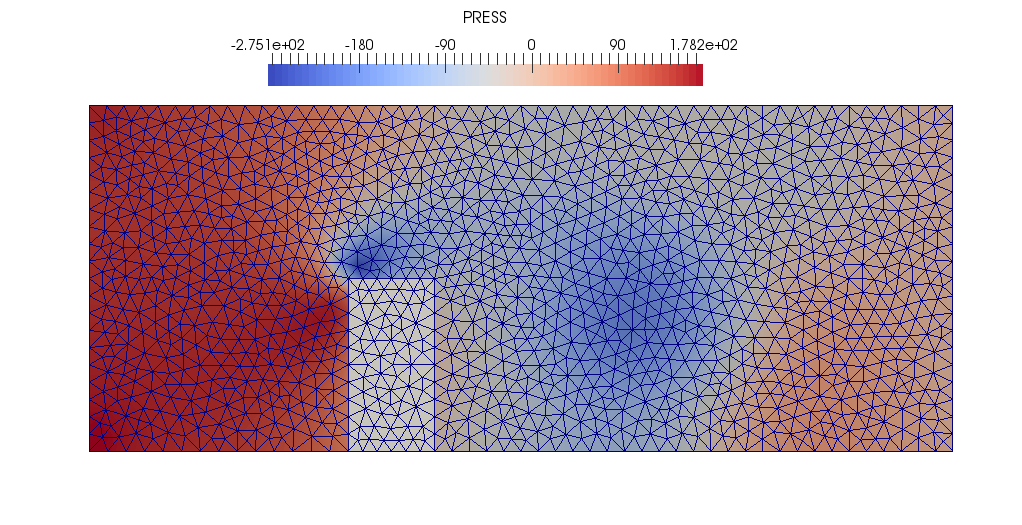
\includegraphics[width=0.5\textwidth]{det_200_firststep}\label{fig:Flap3Det1}}
  \hfill
  \subfloat[Deterministic simulation at time-step 200]{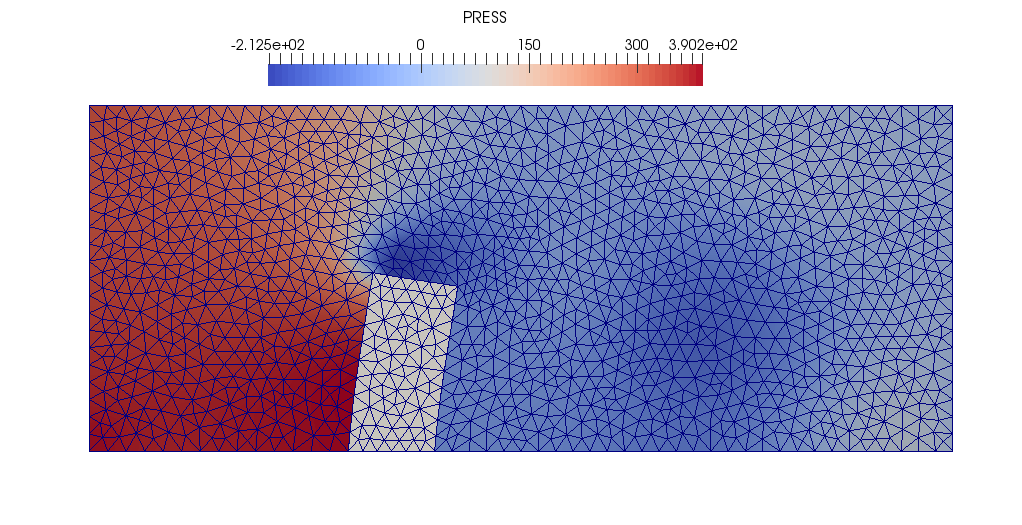
\includegraphics[width=0.5\textwidth]{det_200_laststep}\label{fig:Flap3Det200}}
  \caption{Deterministic simulation of the vertical flap}
  \label{Flap3Det}
  \vspace{-0.4cm}
\end{figure}
The first and the last time step of the deterministic simulation are presented in \refFigure{Flap3Det}, where the visualized fluid's physical parameter was its \emph{pressure}. 

	In the following, the results obtained after the UQ simulations were performed are presented. The next section describes the \emph{one-dimensional} stochastic cases, while the following ones treat \emph{multi-dimensional} scenarios.
\subsection{One Dimensional UQ Simulation}
\label{subsec:1D UQ Simulations}
		
	As the deterministic case was the first important step in the entire set of simulations, the first milestone for the UQ simulations were the \emph{one dimensional} cases. This means that throughout a simulation, \emph{four} out of the \emph{five} input physical parameters are taken to be \emph{sure variables}\footnote{a sure variable is defined to be \emph{exactly determined by given conditions}, i.e. \emph{deterministic}} (see  \cite{Le02} for details), with the fifth being considered to exhibit \emph{uncertainty}. Given the number of input parameters, all five one-dimensional cases were simulated. This means that for the one-dimensional case, an \emph{exhaustive} treatment of uncertainty was made, paving the way for multi-dimensional simulations, as it is explained later in this section. Moreover, for a comprehensive testing and assessment of the employed methods, multiple \emph{configurations} were accounted. First, the variables taken to exhibit uncertainty were modelled as \emph{normal} random variables, and were propagating in the underlying system using both Monte Carlo Sampling and Stochastic Collocations. Afterwards, they were modelled as \emph{uniform} random variables and propagated using Stochastic Collocations. A more detailed presentation is done in the following.
	
	As a starting point, uncertainty is modelled as a \textit{normal random variable} $\Omega$ of the form:
\begin{equation} \label{1DSCGaussian}
\Omega \sim \mathcal{N}(\mu, \sigma^2), \text{with } \sigma = 0.1\mu
\end{equation}
	The first used method was Stochastic Collocations and in order to carry out simulations, the \emph{quadrature degree} (denoted here by \emph{q}) and the \emph{number of coefficients} (denoted here by \emph{n}) have to be established. Based on the maximal implemented q, i.e. ten (c.f. \refSection{sec:Pre-processing}) and the suggested  \emph{rule of thumb} from \cite{Su08}, which states that $q \leq 2 n$, the established combination for this work is \emph{q = 8} and \emph{n = 5}.
\insertfigure{mean_onedim}{Mean for one dimensional scenarios}{fig:SCMeanOnedim}{0.6} % Filename, Caption, Label, Width percent of textwidth
The first processed data sets were the ones corresponding to the \emph{watch point}, which in this case is the upper right corner. Moreover, the quantities of interest were chosen to be the \emph{x axis displacement}, \emph{x axis force} and \emph{y axis force}. 
\insertfigure{var_onedim}{Variance for one dimensional scenarios}{fig:SCVarOnedim}{0.6} % Filename, Caption, Label, Width percent of textwidth 
In \refFigure{fig:SCMeanOnedim} and \refFigure{fig:SCVarOnedim}, the \emph{means} and \emph{variances} of the gathered data are presented, with the means plot including the \emph{deterministic} data as well. From these two plots, several inferences can be made. As a starter, from the first plot, it can be seen that the means of the simulated scenarios almost coincide with each other and even more, are  almost identical to the deterministic data, except for data corresponding to the \emph{Young's modulus}, which, after about time step 80, behaves a little different for the force on the x axis. This outlines two important inferences: first, \emph{on average}, the behaviour is \emph{similar} to the deterministic case and second, \emph{Young's modulus} seems to be the parameter whose uncertainty influences the most the outcomes. Although the plot of the expected values offered the first insights, the \emph{variances} plot is even more interesting, because, among others, it indicates which parameters are important from an uncertain point of view. First of all, it can be seen that, as the variances of the forces exhibit \emph{oscillatory} behaviour, with the one for the y axis force more attenuated, the variance of the x axis displacement increases over time, reaching the peak around time step 190, in the underlying scenario of 200 simulated steps. Moreover, among the five physical parameters, two of them stand out: \emph{fluid's density} and \emph{structure's Young modulus}. From the last observation, it can be pointed out that for the two dimensional case it is expected that combinations including these parameters should have a big impact on the outcomes.

	The results obtained using Stochastic Collocations and normal random variables were compared with the ones output by Monte Carlo Sampling. Considering the high computational and storage demand of this method, a number of \emph{100 samples} were simulated and to quantify the resulting difference, the \emph{mean squared error} (m.s.e.) of the means and variances was computed. 
\begin{table}[h!]
\centering
 \begin{tabular}{|c|c|c|c|} 
 \hline
 statistic & x axis displacement m.s.e. & x axis force m.s.e. & y axis force m.s.e. \\
 \hline 
 mean & 6.238e-10 & 4.974e-4 & 2.737e-4 \\
 \hline 
 variance & 9.603e-14 & 4.359e-4 & 1.436e-4 \\
  \hline
 \end{tabular}
 \caption{Mean squared error for fluid's viscosity}
 \label{table:MCS_SCS_mse}
\end{table}
The comparison was made when the stochastic parameter was \emph{fluid's viscosity}. The statistics plot is outlined in \refFigure{MCS_SCS_com}, whereas the corresponding mean squared errors are presented in \refTable{table:MCS_SCS_mse}.
\begin{figure}[htbp]
  \centering
  \subfloat[Mean comparisson]{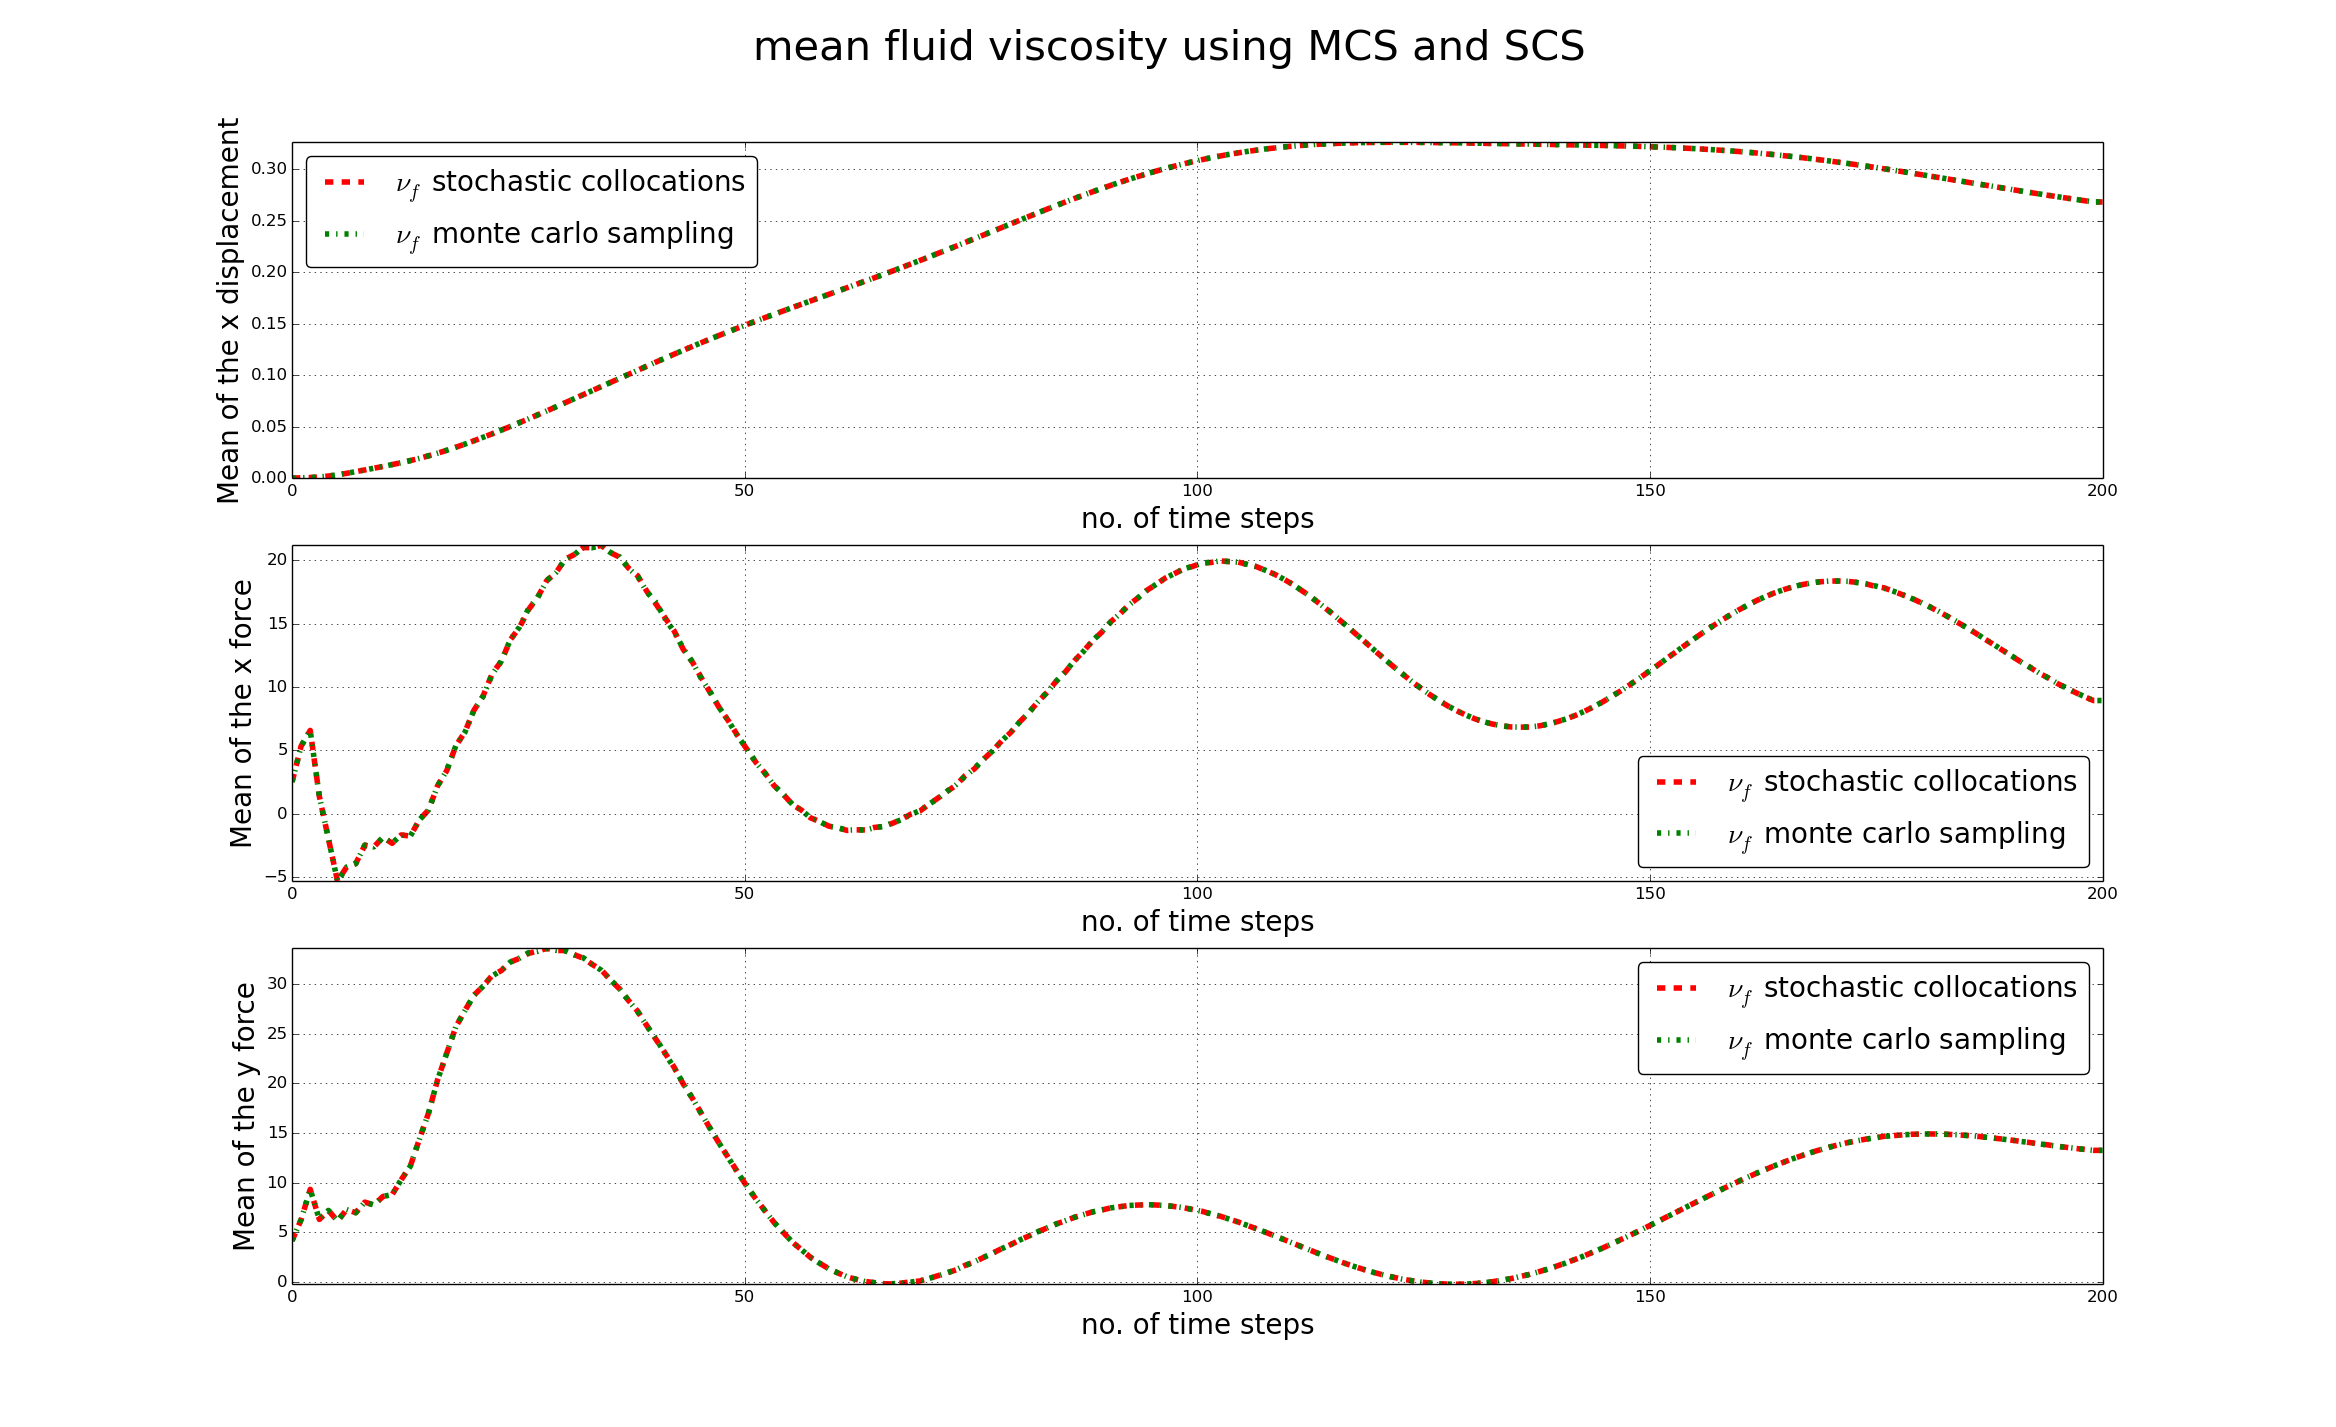
\includegraphics[width=0.5\textwidth]{mean_MCS_SCS_comp}\label{fig:MCS_SCS_mean}}
  \hfill
  \subfloat[Variance comparisson]{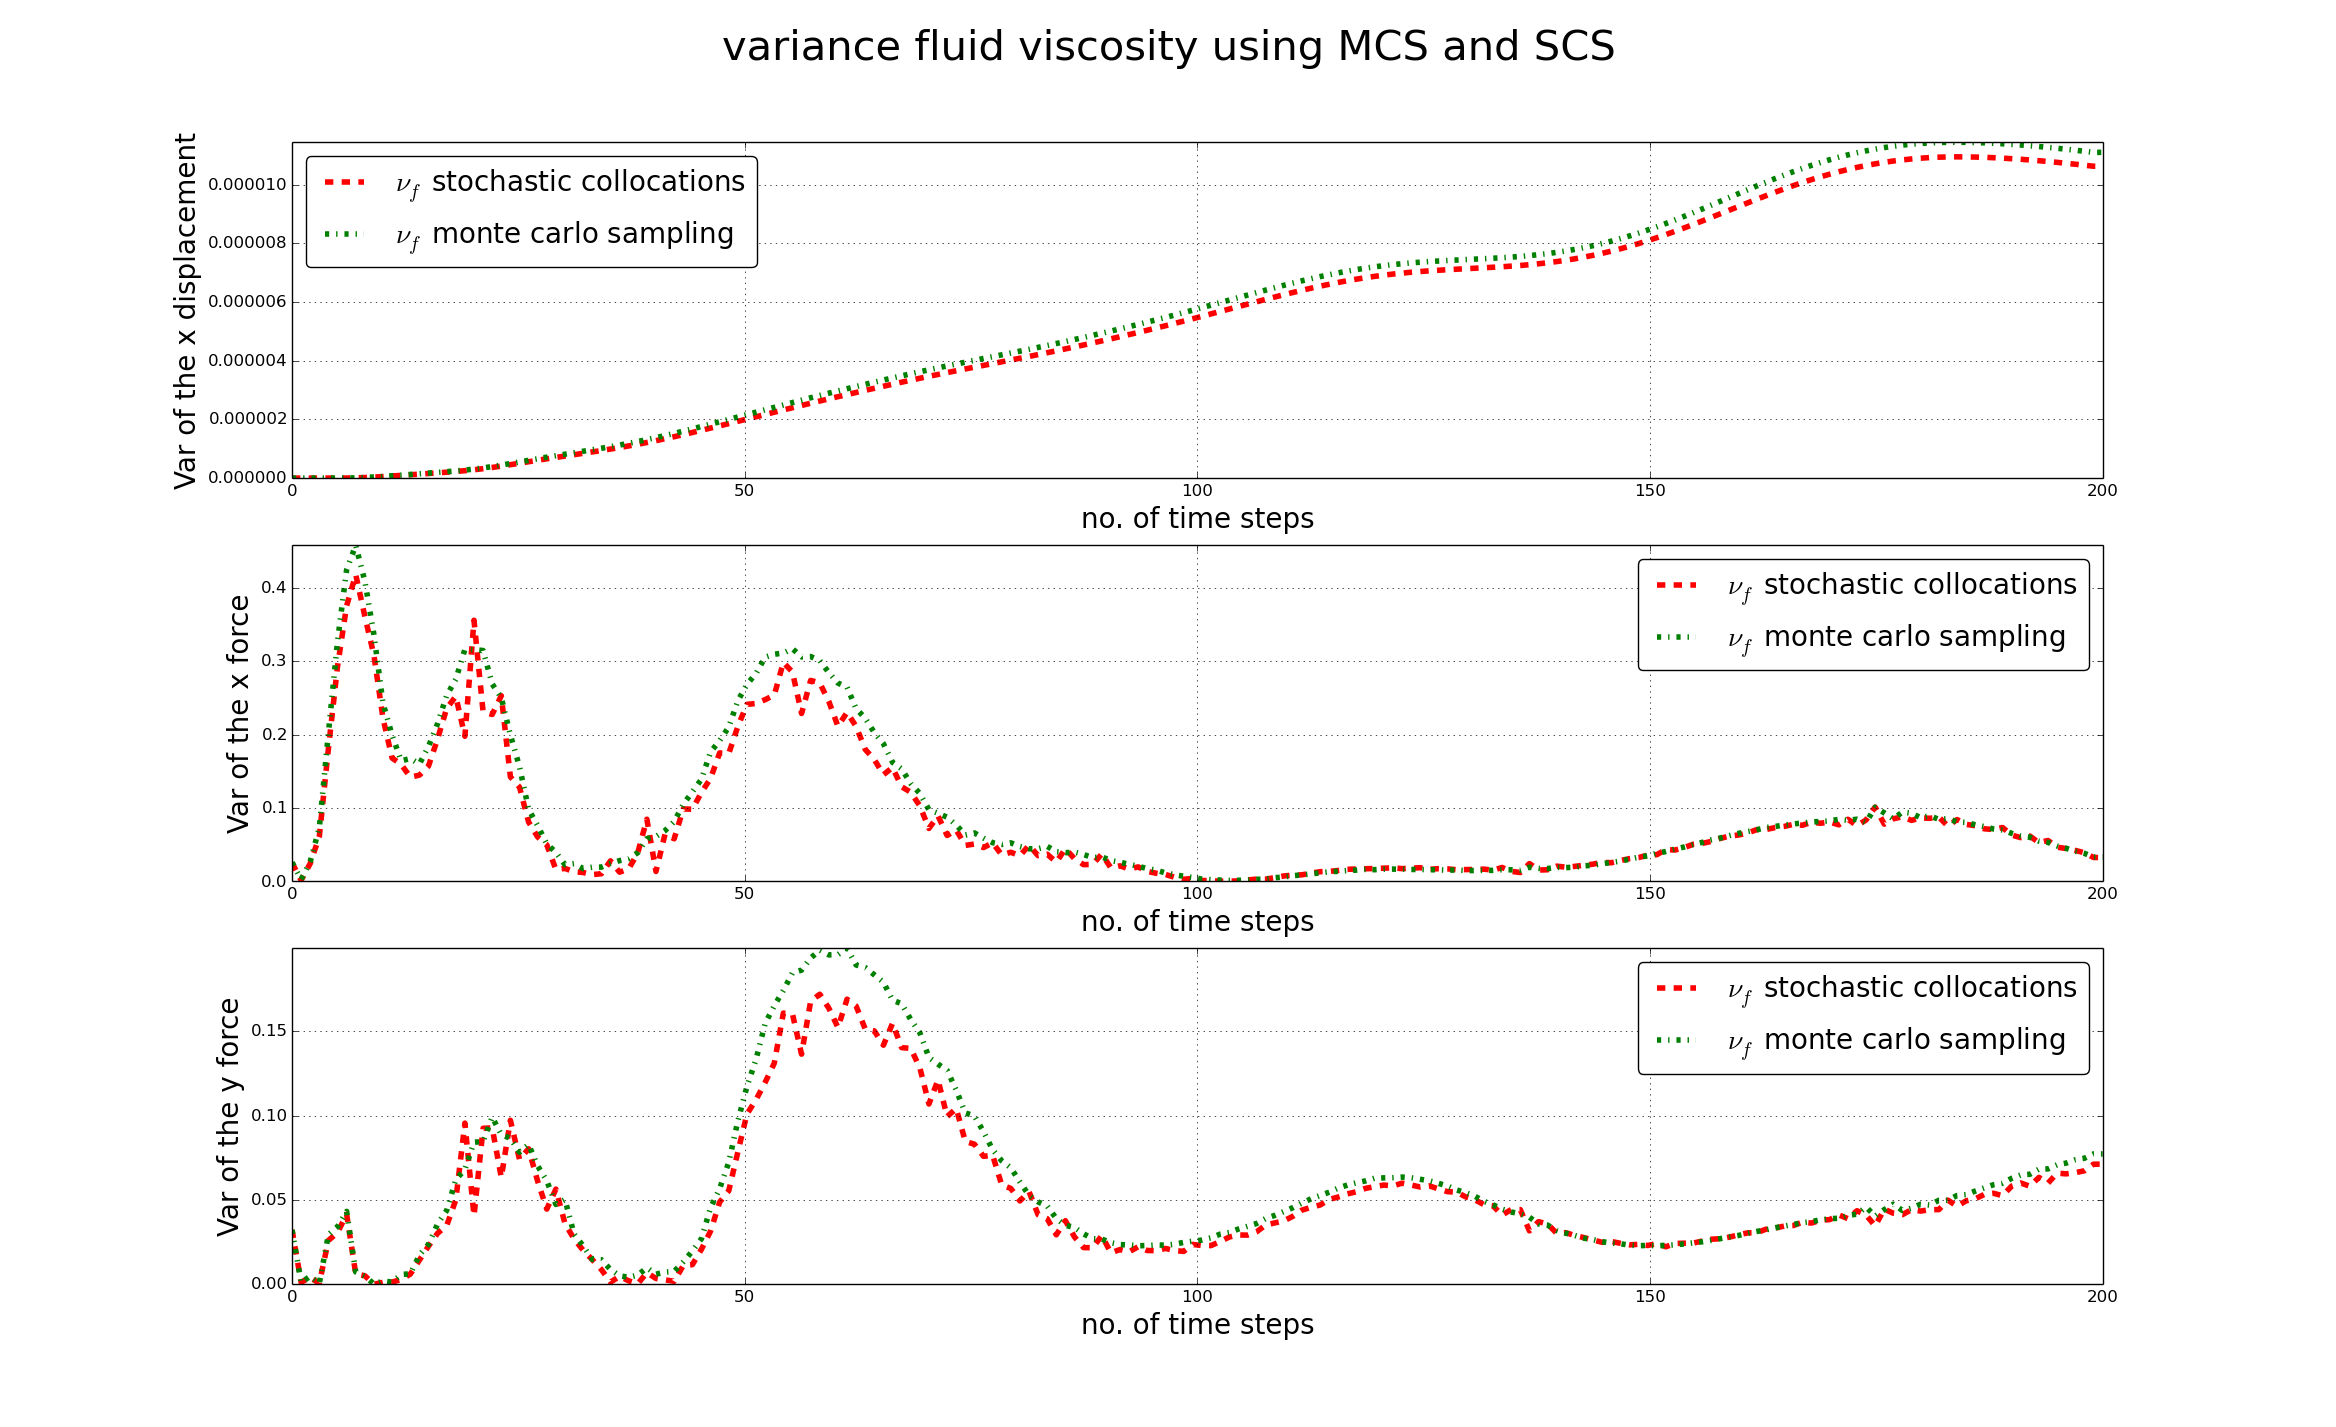
\includegraphics[width=0.5\textwidth]{var_MCS_SCS_comp}\label{fig:MCS_SCS_var}}
  \caption{Comparison of results obtained with both algorithms for fluid's viscosity}
  \label{MCS_SCS_com}
  \vspace{-0.4cm}
\end{figure}
Based on these results, it results that Stochastic Collocations with a quadrature degree of order 8 and 5 expansion coefficients converges. Moreover, similar results were obtained when testing for the other four parameters and hence, ascertaining the previous assertion.

	The next step was to get a better understanding of how the normal distribution affects the outcomes. To this extent, based on \refEquation{1DSCGaussian}, the uncertain parameters were modelled as \emph{uniform random variables} $\Gamma$ of the form:
\begin{equation} \label{1DSCUniform}
\Gamma \sim \mathcal{U}(a, b), \text{with } a = 0.9\mu \text{ and } b = 1.1\mu, 
\end{equation}
where $\mu$	is the mean used for normal random variables. As with Monte Carlo Sampling, the comparison was made when the stochastic parameter was \emph{fluid's viscosity}. The statistics plot is outlined in \refFigure{SCS_com} and the corresponding mean squared errors are presented in \refTable{table:SCS_nor_uni_mse}.
\begin{table}[h!]
\centering
 \begin{tabular}{|c|c|c|c|} 
 \hline
 statistic & x axis displacement m.s.e. & x axis force m.s.e. & y axis force m.s.e. \\
 \hline 
 mean & 1.049e-8 & 9.987-4 & 5.072e-4 \\
 \hline 
 variance & 1.244e-14 & 4.737e-4 & 1.568e-4 \\
  \hline
 \end{tabular}
 \caption{Mean squared error for fluid's viscosity}
 \label{table:SCS_nor_uni_mse}
\end{table}
\begin{figure}[htbp]
  \centering
  \subfloat[Mean comparisson]{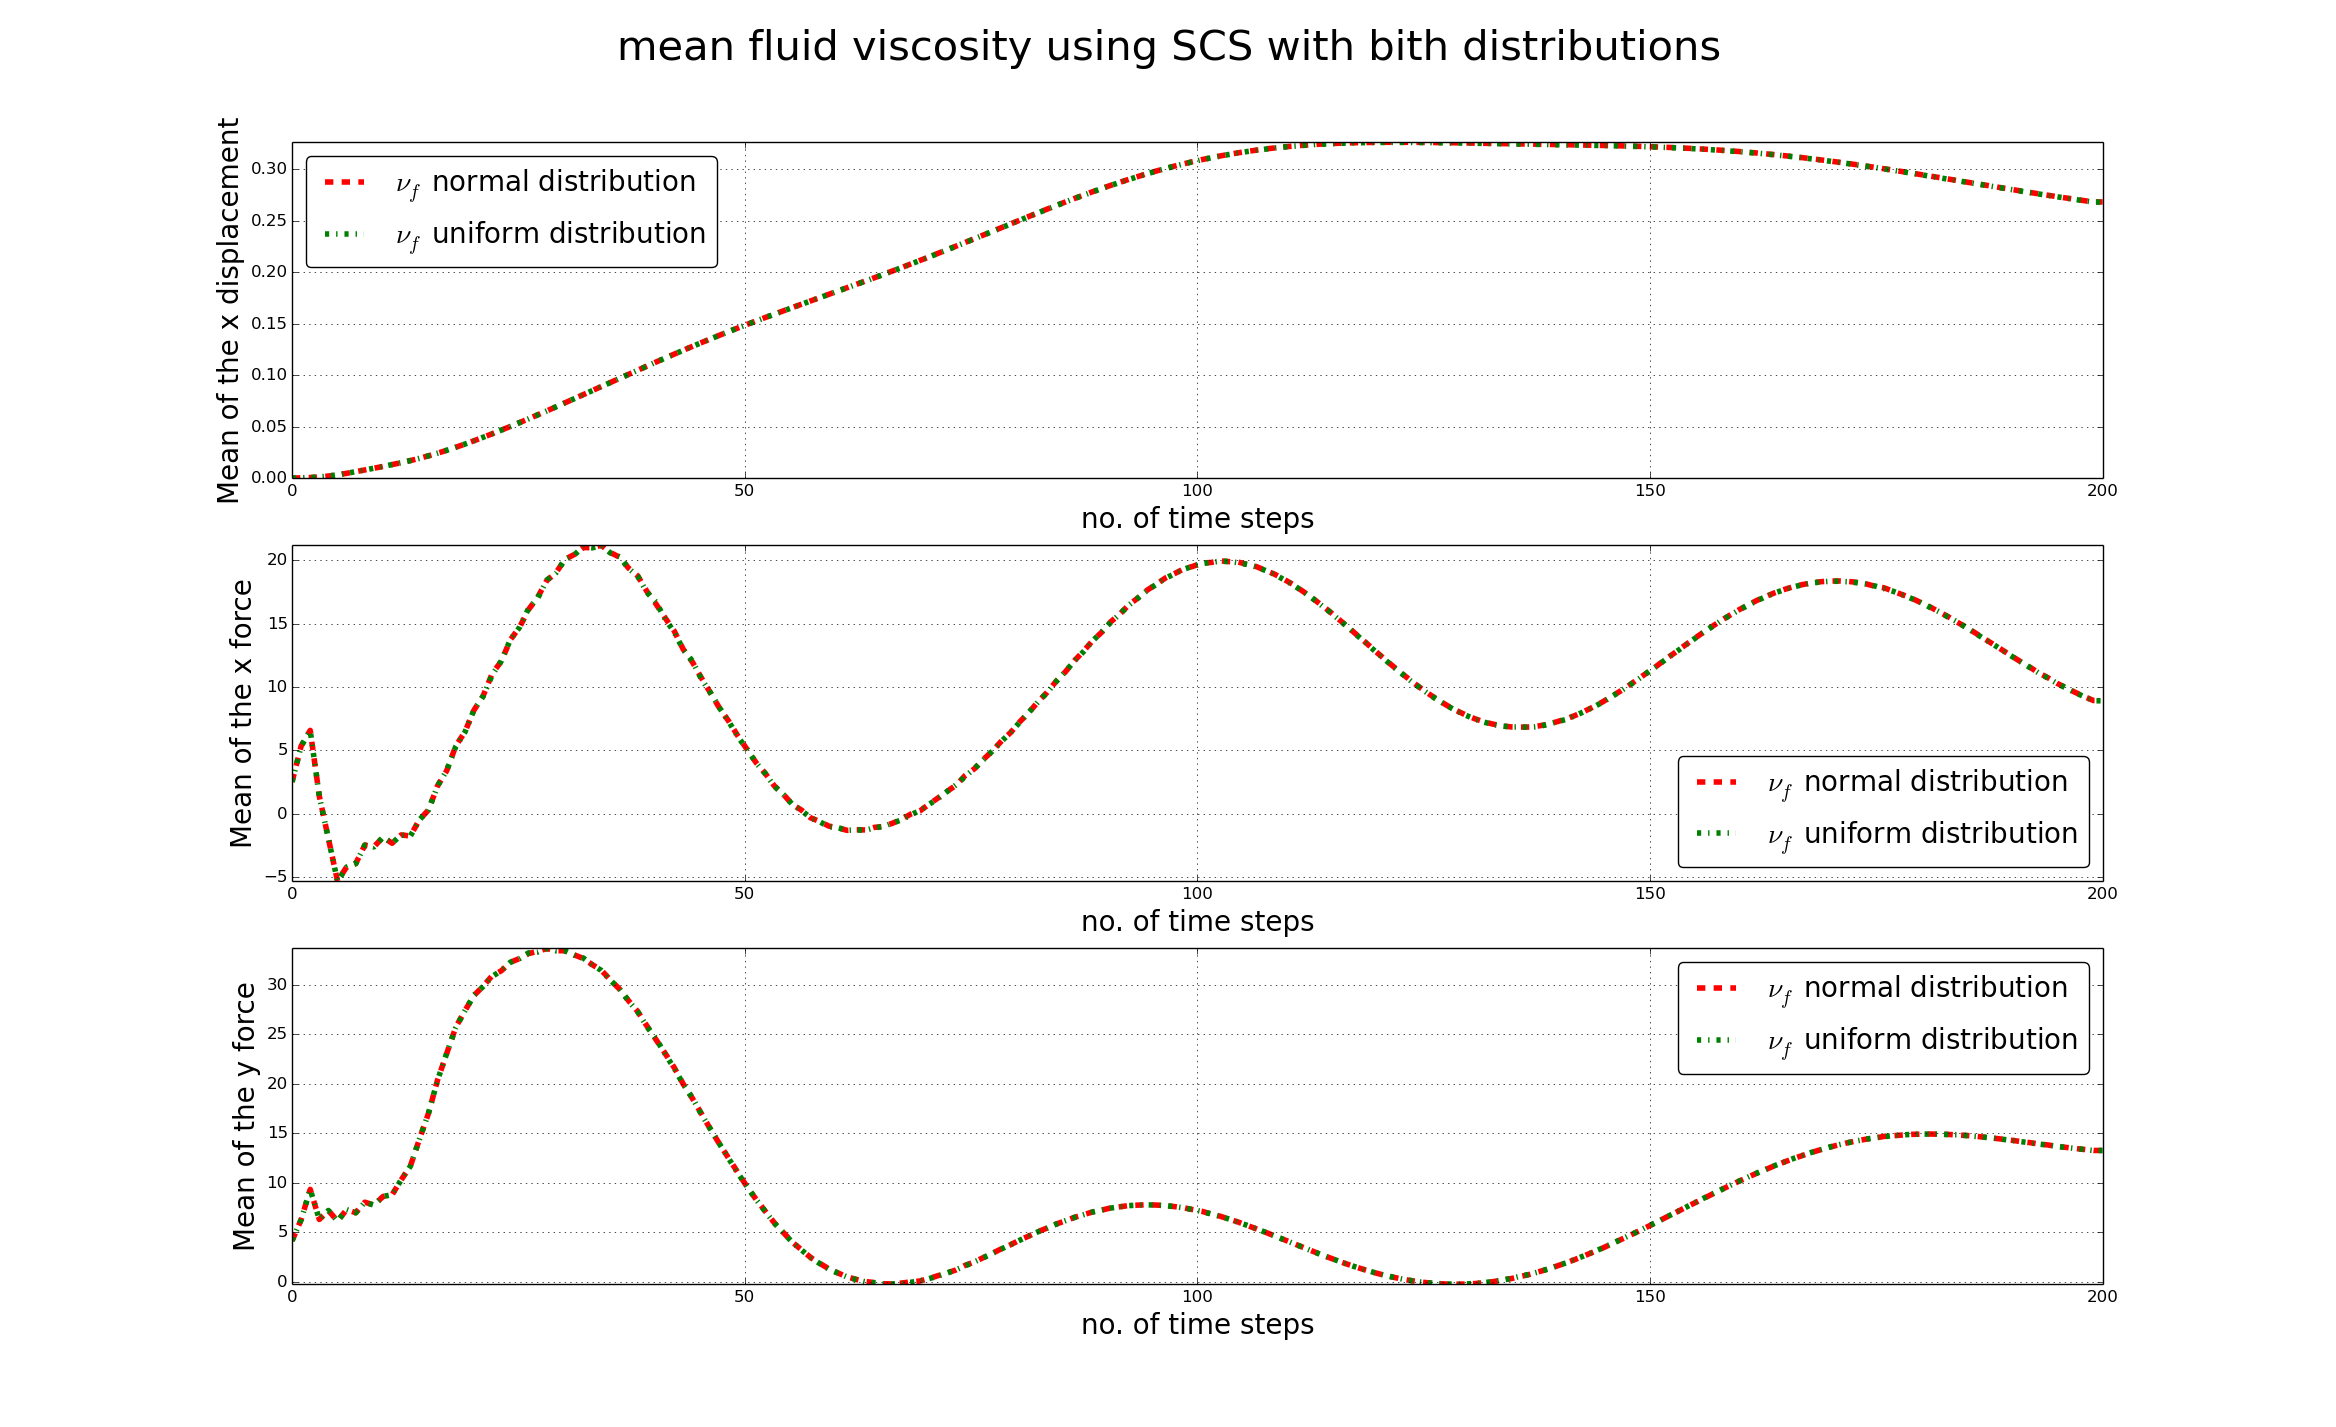
\includegraphics[width=0.5\textwidth]{mean_SCS_comp}\label{fig:SCS_nor_uni_mean}}
  \hfill
  \subfloat[Variance comparisson]{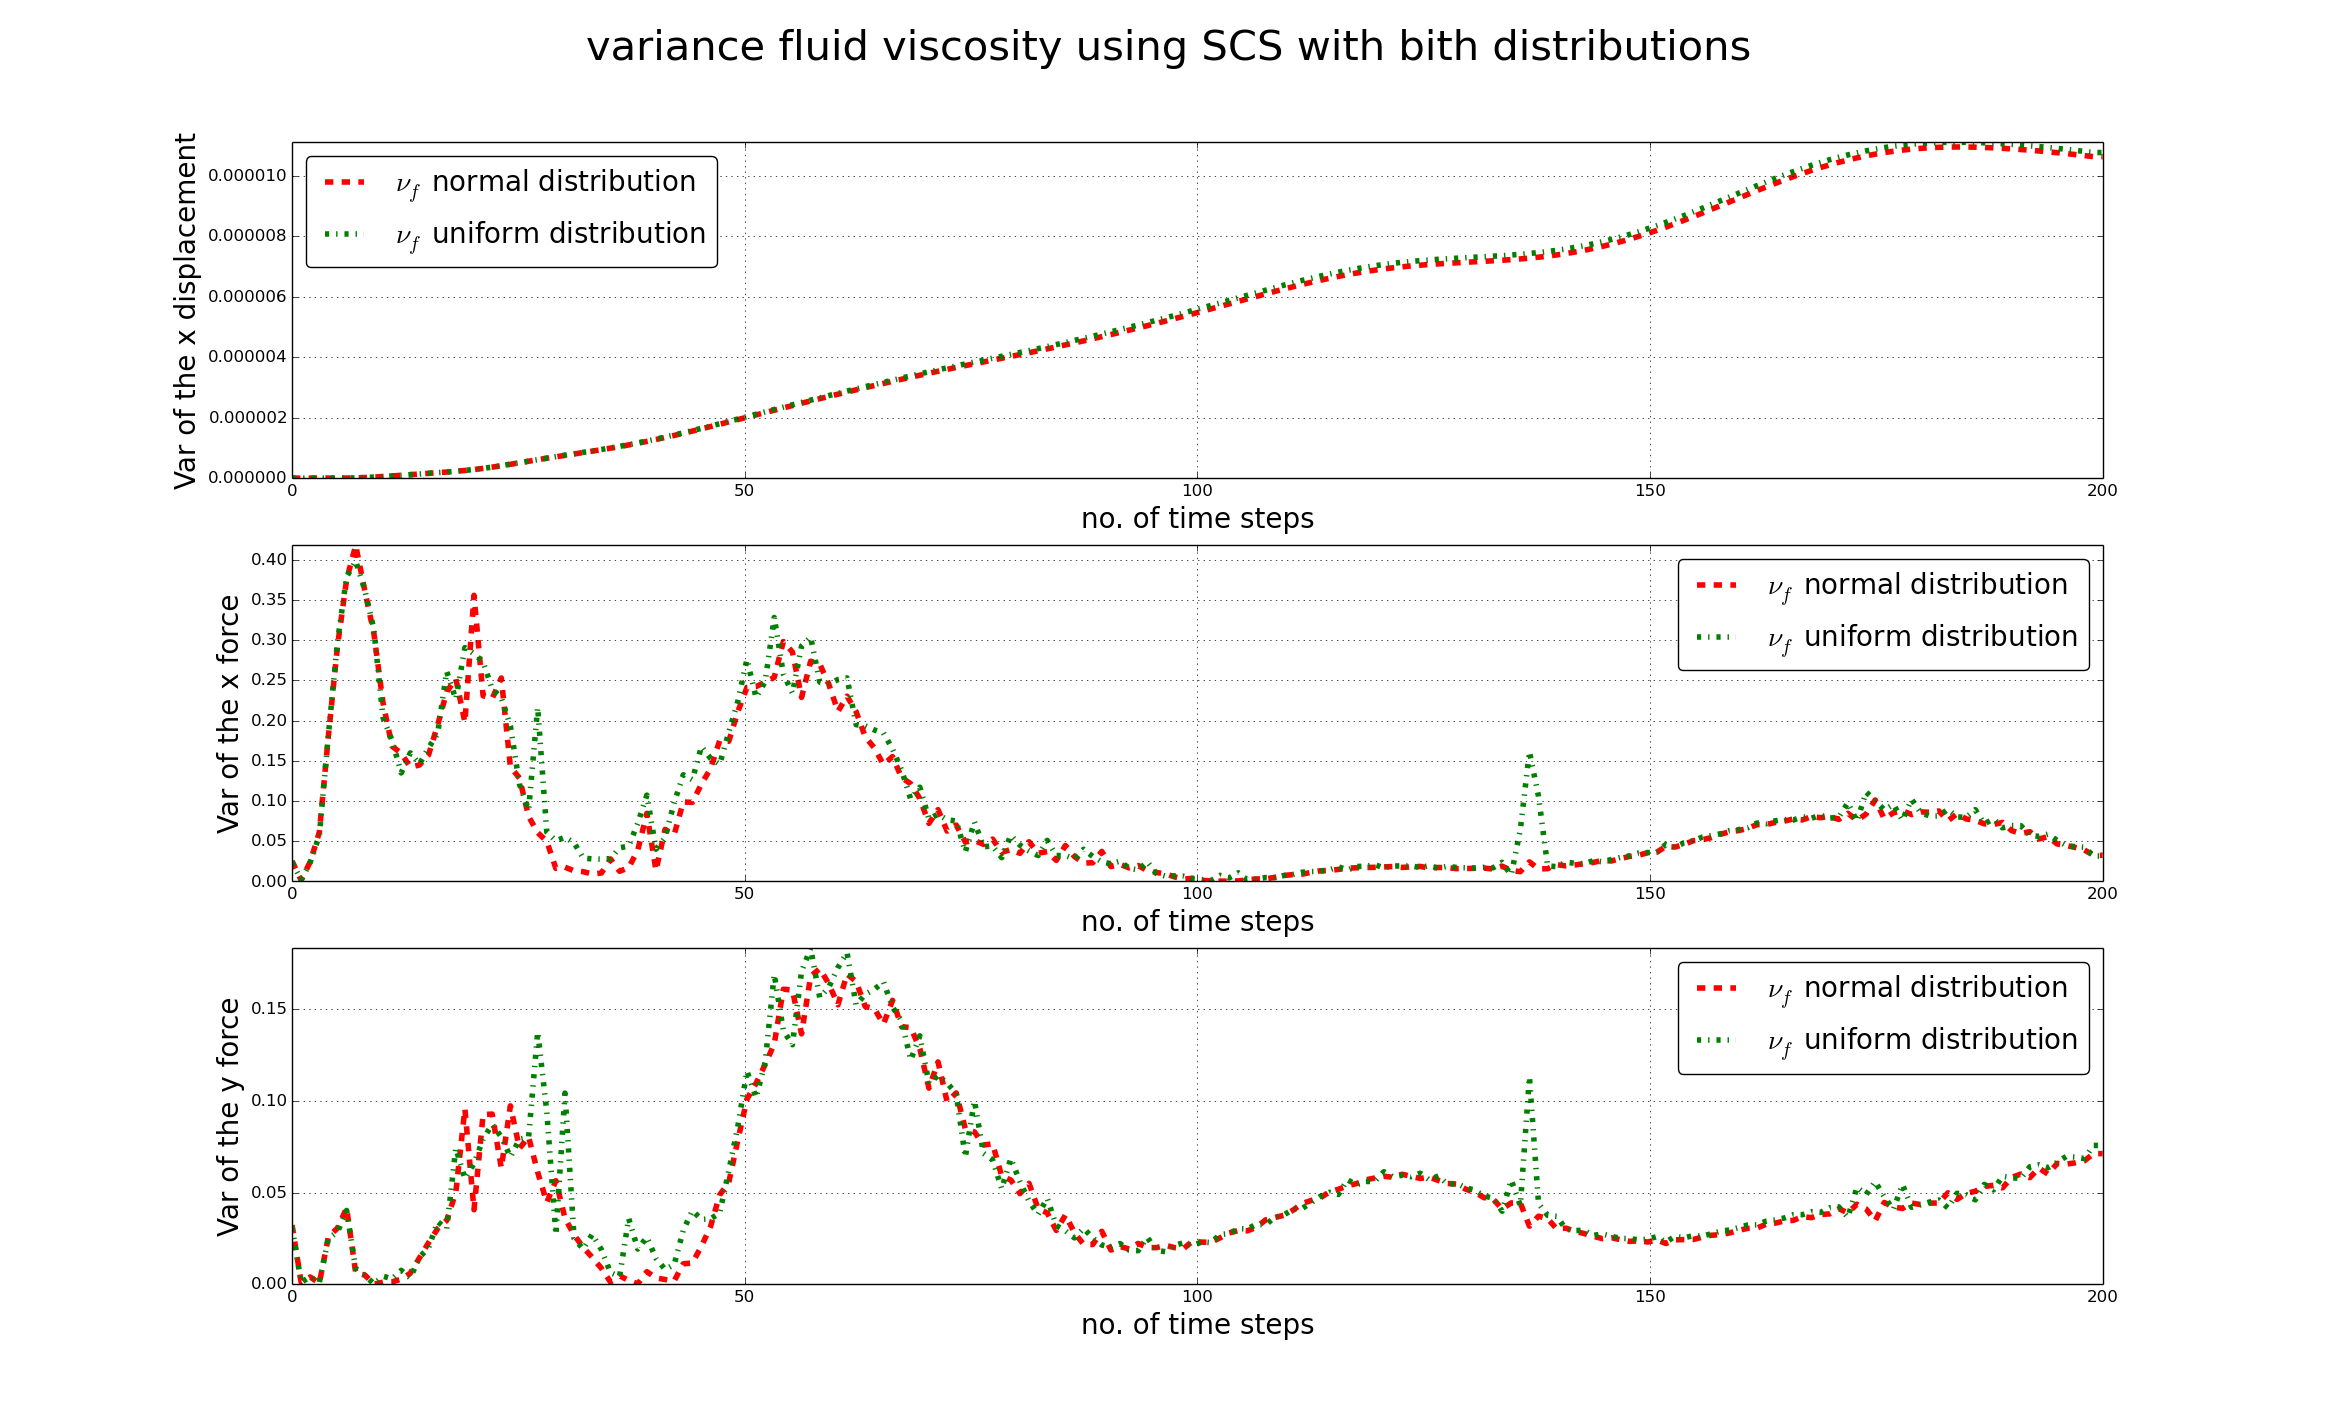
\includegraphics[width=0.5\textwidth]{var_SCS_comp}\label{fig:SCS_nor_uni_var}}
  \caption{Comparison of results obtained with normal and uniform for fluid's viscosity}
  \label{SCS_com}
  \vspace{-0.4cm}
\end{figure}
Likewise Monte Carlo Sampling, the results obtained by using uniform random variables were very similar to the case when using normal random variables. Even more, similar results were obtained for the other four parameters as well. 

	Based on these results, it follows that Stochastic Collocations with normal random variables as in \refEquation{1DSCGaussian}, is enough for performing uncertainty propagation in the underlying scenario. That is why, in the following, only results outlined by this strategy are presented. 
\subsection{Two Dimensional UQ Simulations}
\label{subsec:2D UQ Simulations}

\subsection{Five Dimensional UQ Simulations}
\label{5D UQ Simulations}

\section{Scenario II - rename}
\label{Scenario II}



